%!TEX root = ../thesis.tex
%*******************************************************************************
%****************************** Third Chapter **********************************
%*******************************************************************************
\chapter{Setting The Upper Limits on The Mixing Angle of HNL}
\label{ChapterResult}

% **************************** Define Graphics Path **************************
\ifpdf
    \graphicspath{{Chapter10/Figs/Raster/}{Chapter10/Figs/PDF/}{Chapter10/Figs/}}
\else
    \graphicspath{{Chapter10/Figs/Vector/}{Chapter10/Figs/}}
\fi

%********************************** %Opening  **************************************

Chapter 9 Opening

\clearpage

%********************************** %First Section  **************************************
\section{Systematic Uncertainties}

\subsection{The Reweighting Method}
\label{sec:reweighting}

%describe reweighting
The impact of systematic uncertainties on a physics measurement can be assessed by simulating and reconstructing a number of different samples, referred to as \textit{universes}, each with a physics parameter tweaked within its uncertainty range.
The physics measurement is then performed in each universe in the same manner as done on the Central Value (CV) sample that does not have any parameters tweaked.
The variation of the result across universes compared to the CV sample describes the uncertainty that the tweaked parameter has on the measurement.
However, fully simulating and reconstructing a large MC sample for multiple systematic parameters can be computationally intensive, the \textit{reweighting} technique is used instead by producing a weight associated with the tweaked parameter per universe.
The weight can be applied to smear the physics result by an amount as expected by the tweaked parameter.
Or vice versa, the smeared physics result can be unweighted to recover the original result without any uncertainties from the tweaked parameter \cite{cowan_stat}.

%define weight
The reweighting technique begins with transforming a physics parameter $x$ to $x'$ as follows
\begin{equation}
	x' = x \cdot f(x)
\end{equation}
where $f(x)$ describes some transformation functions as a function of $x$. 
If $f(x) = 1$, then $x'$ is equal to the unweighted $x$.
A common form of the transformation function  is a Gaussian function, where the physics parameter $x$ is thrown to $x'$ by randomly sampling from a unit Gaussian with its mean and sigma is set as 1.
Another common formalism is the Delta function, where $x'$ can take only take the value of 0 or 1. 

%\begin{equation}
%	x' = x \times f\left( 1 + n_\sigma \frac{\sigma_x}{x} \right)
%\end{equation}
%where $\sigma_x$ is the standard deviation of $x$ and $n_\sigma$ is the number of standard deviations to shift the parameter $x$.
%If $n_\sigma = 0$, then $x'$ is equal to the unweighted $x$.

Then, from the probability $P(x)$ describing some physic properties parameterised by the physics parameter $x$, the weight $w$ can be computed as
\begin{equation}
\label{eq:prob_w}
	w = \frac{P(x')}{P(x)}
\end{equation}
%TODO: Add stuff and weight computing from multisim/multisigma/unisim
The weight $w$ describes whether the probability $P(x')$ is more or less likely to occur given the transformed parameter $x'$ compared to the CV parameter $x$.
The distribution of $w$ therefore describes the Probability Density Function (PDF) of the parameter $x$.
A universe associated with a weight $w$ represents an outcome sampled from the PDF.
The weight example shown in Eq. \ref{eq:prob_w} is associated with a single physics parameter non-correlated to any other parameters, however, a weight associated with multiple correlated parameters can also be computed in the same manner.

The reweighting framework provides a quick way to compute the PDFs, allowing for the assessment of the impact of systematic uncertainties without the computational expense of simulating and reconstructing the sample multiple times.
A series of universes is first simulated and weights for every interaction, whether SM neutrino or HNL, are then calculated from the PDFs for each universe.
The variation of the physics result across universes are used to quantify the uncertainties of the weighted physics parameters have on the physics measurement, of which the error propagation is formalised in Sec. \ref{sec:error_prop}.  

%detector systematic
In some cases, reweighting is not applicable such as evaluating uncertainties due to detector effects.
For example, recombination, as detailed in Sec. \ref{sec7:delta}, influences not only the charge and light yield but also the charge deposition on wires non-uniformly. 
Consequently, it is non-trivial to quantify analytically the downstream impacts due to the variation in recombination parameters on the charge reconstruction by Pandora or any high level analysis tools using the reconstructed charge information.
A full simulation and reconstruction of a single universe using the varied recombination parameters is needed to fully assess the impact on the physics measurement. 
This method is commonly used for detector systematic uncertainties.

\subsection{Error Propagation Formulation}
\label{sec:error_prop}

The impact of uncertainties can be evaluated by constructing the covariance matrix $V$ of a series of observations $N$.
The matrix describes the average deviation of the value in bins $i$ and $j$ from the CV away from the universe $n$, totalling $U$ universes.
The matrix is computed as follows
\begin{equation}
	V_{ij} = \frac{1}{U}\sum^{U}_{n} \left( N^n_{i} - N^{CV}_{i} \right) \left( N^n_{j} - N^{CV}_{j} \right)
\end{equation}
The diagonal term of the covariance matrix represents the variance in a given bin and the error $\sigma$ can be derived as
\begin{equation}
\label{eq:diag_cov}
	V_{ii} = \sigma^2_i
\end{equation}

Since there are multiple sources of error, as detailed in the forthcoming sections, the total covariance matrix is computed by summing the covariance matrix from each error source together, effectively adding the errors in quadrature as follows
\begin{equation}
	V^{Total}_{ij} = \sum_{Sources} V_{ij}^{Source} = V_{ij}^{Stat} + V_{ij}^{Flux} +V_{ij}^{Cross\ Section} + ...
\end{equation}
The total error is then computed from the total covariance matrix using Eq. \ref{eq:diag_cov}.
Additionally, the fractional matrix describing the relative error in each bin is computed, allowing for easy and direct comparison across bins of signal and background samples. 
\begin{equation}
	V_{ij}^{Frac} = \frac{V_{ij}}{N_i^{CV}N_j^{CV}}
\end{equation}

\subsection{Signal Uncertainty Sources}
\label{sec:signal_error}

For the HNL signal, there are four primary sources of uncertainties that will effect physics measurements by SBND: (1) statistical, (2) cosmic mis-tagging, (3) flux and (4) detector . 
The statistical uncertainty is evaluated using the number of signal slices selected after the selection presented in Chapter \ref{ChapterSelect}.
Meanwhile, the cosmic mis-tagging uncertainty is evaluated using the number of cosmic muon slices occurring in the same readout window of HNLs.
The impact of the uncertainties due to flux modelling can be measured using the reweighting method.
The detector systematic however is not reweightable and requires a full simulated and reconstructed MC sample for assessing uncertainties due to detector as previously explained in Sec. \ref{sec:reweighting}.
At the time of writing, the SBND detector is not yet operational, and thus, it is undetermined which detector parameters are impactful on physics measurements.
Thus, detector systematics are not included in the limit setting presented here, but should be included in future iterations of this analysis.

The statistical uncertainty describes the statistical fluctuation due to the MC sample.
It is computed using the number of HNL signal slices remained after the selection binned to the beam bucket distribution.
The statistical uncertainty of each bin of the distribution is defined as follows 
\begin{equation}
\label{eq:stat_err}
    \sigma_{statistics} = \sqrt{Number\ of\ entries\ in\ the\ bin}
\end{equation}
The uncertainty is computed before the normalisation to the target POT exposure of 3 years data taking.
After the normalisation, the resulting statistical uncertainty is plotted in Fig. \ref{fig:hnl_stat}, showing the uncertainty is minimal across the entire distribution.
The fractional statistical uncertainty, as shown in the blue line in the bottom figure of Fig. \ref{fig:hnl_total_error}, shows that it is is well-constrained under $< 6\%$.

The cosmic mis-tagging uncertainty is to account for the selected slices that are cosmic rays occurring in the same readout window as HNLs.
In some cases, high energetic cosmic rays can overlap with showers from HNLs, resulting in a pile-up of charge clusters at the same location in the detector.
Drifting electrons arriving at the same wires and at the same time can mislead the clustering process of Pandora during reconstruction, such that a reconstructed shower object might contain more charges from cosmic rays then HNLs.
This reconstruction failure results in a number of cosmic slices remained after the selection, and therefore, is considered as the cosmic mis-tagging uncertainty.
The cosmic mis-tagging uncertainty is plotted in Fig. \ref{fig:hnl_mistag}, however, the uncertainty is so small that it is not visible on the plot.
The uncertainty can be seen in the fractional formalism in the bottom figure of Fig. \ref{fig:hnl_error} in the gray line, demonstrating it is almost negligible at $< 1\%$. 

The flux systematic was assessed using the reweighting method.
The flux prediction and the reweighting framework for assessing the uncertainties were both developed by the MiniBoonE experiment and implemented for SBND.
%TODO: add appendix
The flux systematic uncertainties are as follows
\begin{coloritemize}
	\item \textbf{Proton Delivery}: The proton intensity on the target of the BNB is measured using two steroids, which have an uncertainty of 2\% attributed to calibration.
	\item \textbf{Production}: The number of secondary mesons produced in the BNB target has an uncertainty associated with each particle type. 
		The model predictions for $\pi^\pm$, $K^\pm$ and $K^0_L$ mesons are previously detailed in Sec. \ref{sec4BNB}.
		The main meson parent of HNLs is $K^+$, of which the production is extrapolated from the global data of $K^+$ using the Feynman Scaling to the relevant BNB energy range, and futher constrained by the SciBooNE's direct measurement of $K^+$ from the BNB.
	\item \textbf{Hadronic Interactions}: Hadrons produced in the target may interact with the Beryllium target elastically or inelastically, effecting the kinematics of secondary mesons and consequently, tertiary daughter particles like HNLs and neutrinos.
		The uncertainty of interaction cross sections of $p/n + Be$ and $\pi^\pm + Be$ is propagated through the flux prediction.
		The
	\item \textbf{Horn Magnetic Field}: The magnetic field of the horn impacts the focusing of charged particles produced in the target.
		Uncertainties associating with the horn magnetic field including the current pulsed through the horn and the skin current induced on the surface of the target are computed.
\end{coloritemize}
Fig. \ref{fig:hnl_flux} shows the combined uncertainty of all the flux systematics listed here for HNLs, where the uncertainty is consistent across every bin.
The flux fractional uncertainty is plotted in the green line in the bottom figure of Fig. \ref{fig:hnl_total_error} that it is well-constrained $< 8\%$.

Finally, the top figure of Fig. \ref{fig:hnl_total_error} shows the total uncertainty combining the statistical, cosmic mis-tagging and flux uncertainties combined.
It can be seen that the uncertainty is evenly distributed across the beam bucket distribution with minimal biases in any bins. 
The total fractional uncertainty is shown in the purple line in the bottom figure of Fig. \ref{fig:hnl_total_error}, showing that it is well-constrained $< 10\%$ across the full distribution.

%TODO: Update plots to after POT
\begin{figure}[htbp!]
        \begin{subfigure}[b]{0.495\textwidth}   
            \centering 
            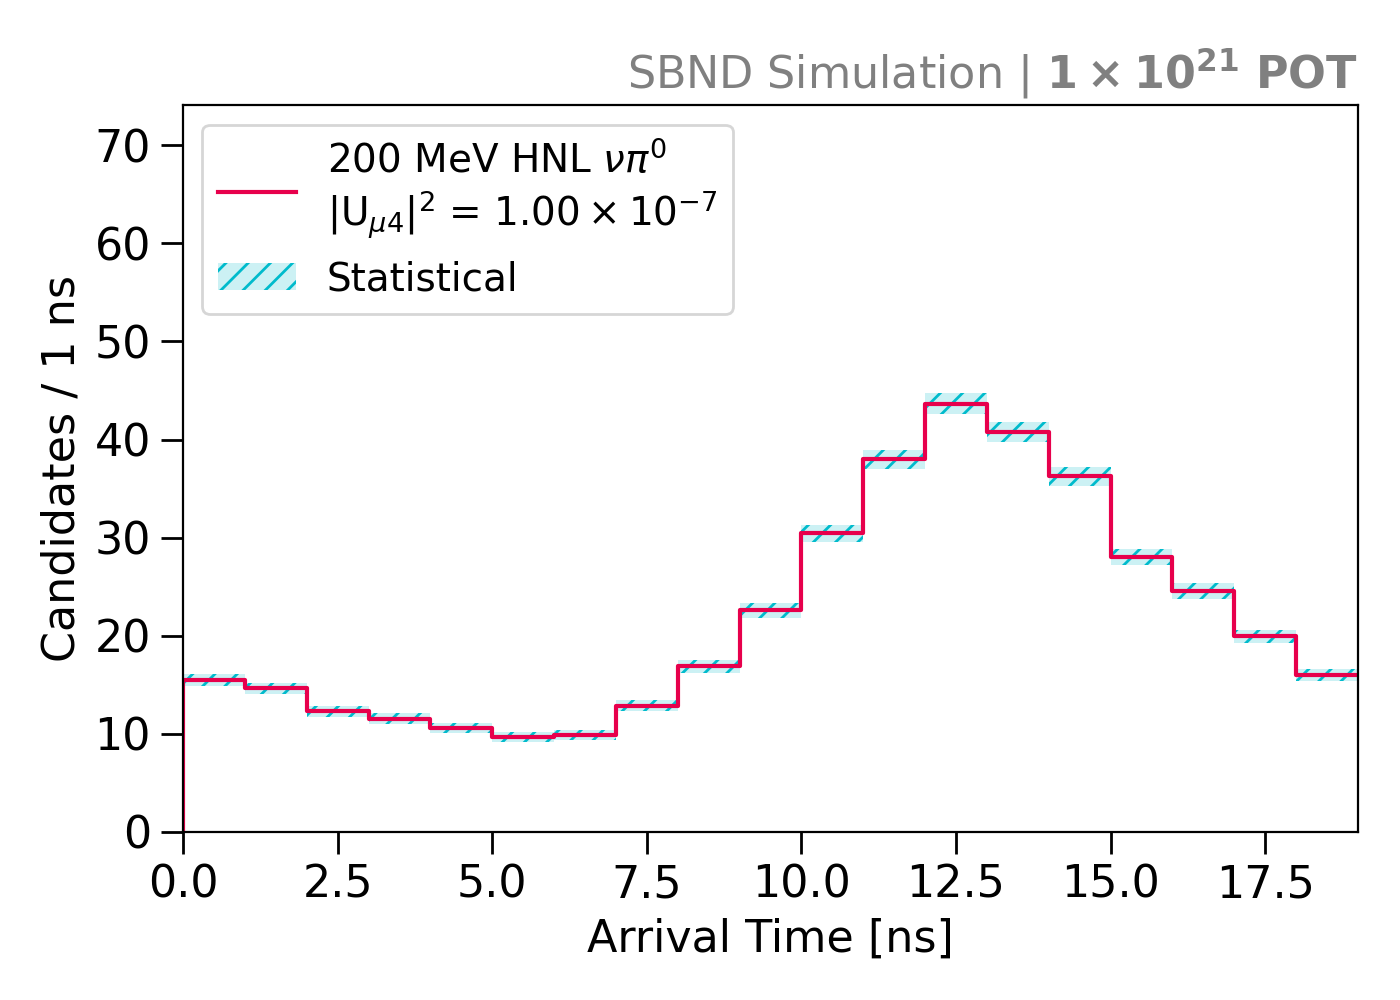
\includegraphics[width=\textwidth]{hnl_statistics_error}
            \caption{Statistical}%
            \label{fig:hnl_stat}
        \end{subfigure}
        \hfill
        \begin{subfigure}[b]{0.495\textwidth}   
            \centering 
            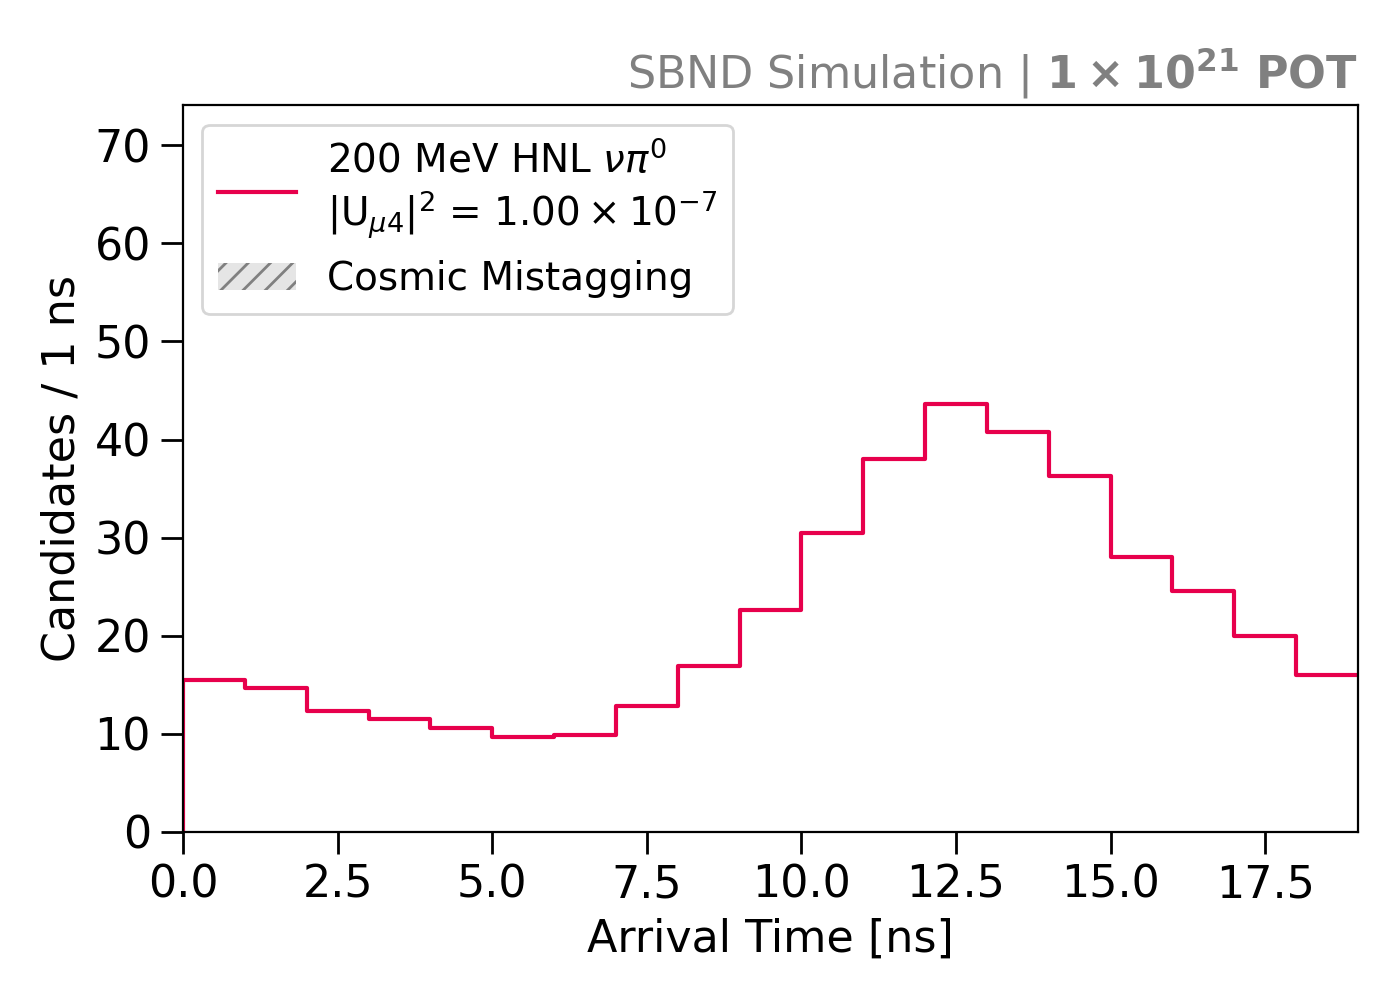
\includegraphics[width=\textwidth]{hnl_mistagging_error}
            \caption{Cosmic Mis-tagging}%
            \label{fig:hnl_mistag}
        \end{subfigure}
        \centering
        \begin{subfigure}[b]{0.495\textwidth}   
            \centering 
            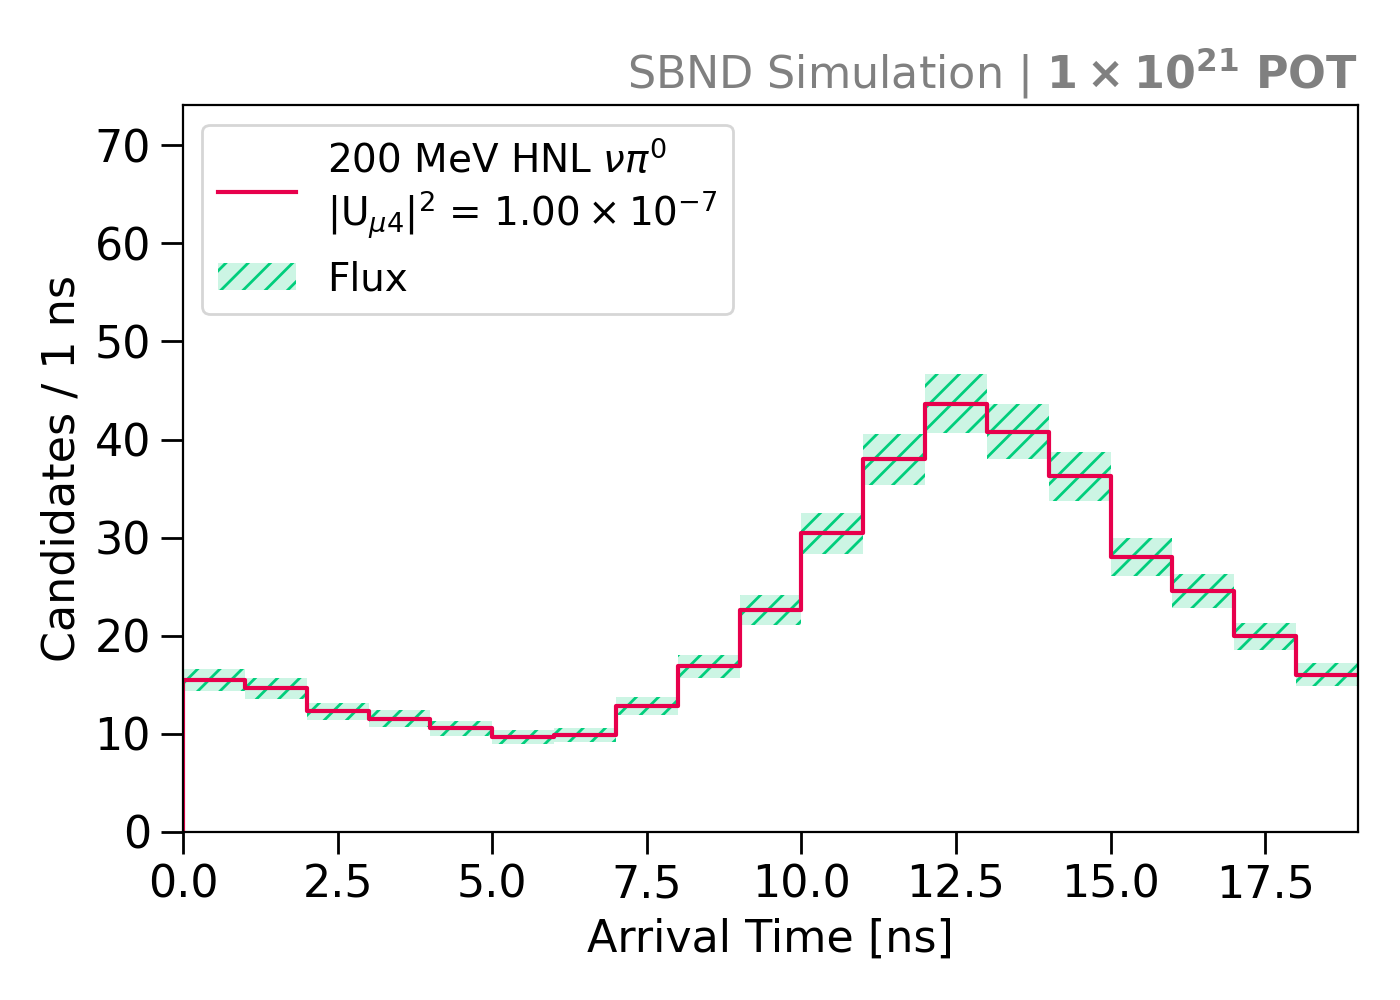
\includegraphics[width=\textwidth]{hnl_flux_error}
            \caption{Flux}%
            \label{fig:hnl_flux}
        \end{subfigure}
        \caption{
	Plot showing different sources of uncertainty (bottom) of HNLs.
	}
        \label{fig:hnl_error}
	\vspace{0.5cm}
%\end{figure}
%\begin{figure}[htbp!] 
\centering    
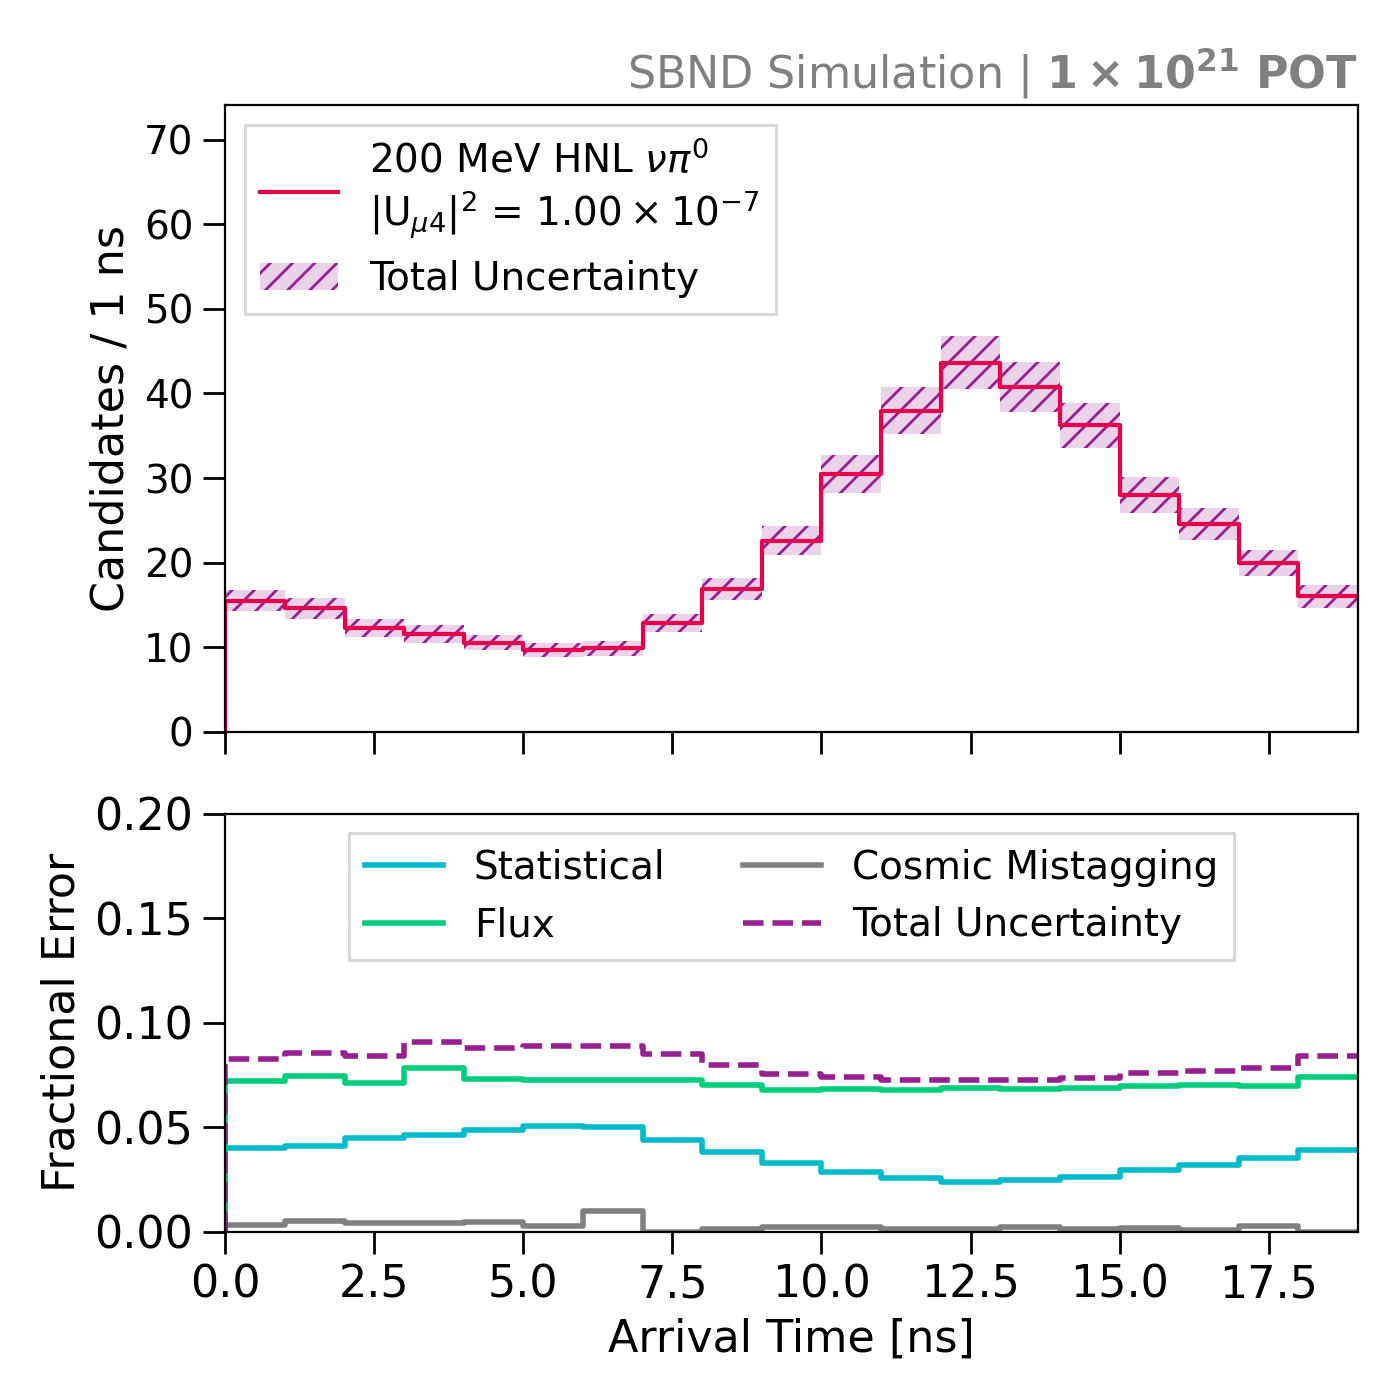
\includegraphics[width=0.5\textwidth]{hnl_error}
\caption[hnl_error]{
Plot showing the total uncertainty (top) and fractional uncertainties (bottom) of HNLs.
}
\label{fig:hnl_total_error}
\end{figure}

\subsection{Background Uncertainties}

For the background of SM neutrinos and cosmic muons, there are four primary sources of uncertainties: (1) statistical, (2) flux, (3) neutrino cross section and (4) detector.
The uncertainties due to statistic and flux are computed in the same manner as the uncertainty treatment of the HNL signal.
The detector systematic uncertainty is also currently not included but should be included in the future work.
A new addition is the neutrino cross section uncertainty, of which the impact due to the cross section modelling is measured using the reweighting method.

The statistical uncertainty of the background was assessed using the number of SM neutrino and cosmic muon slices after the selection.
The statistical uncertainty of each bin is computed using Eq. \ref{eq:stat_err}.
The statistical uncertainty of background is shown in Fig. \ref{fig:bkg_stat}.
It is evident that the background statistics is abundant for bins at the centre of the beam bucket however, limited for bins at the edge.
Therefore, the statistical uncertainty is better constrained for bins at the centre, while bins at the edge have a higher statistical fluctuation.
This is visually evident in the statistical fractional uncertainty plotted in the blue line in the bottom figure of Fig. \ref{fig:bkg_total_error}.
For bins at the centre of the beam bucket, the statistical fractional uncertainty is constrained at $< 20\%$ while, for bins the edge of the beam bucket distribution, particular the first and last 4 bins, where the statistical fractional uncertainty reaches as high as $100\%$.

The flux systematic of the background was measured using the reweighting method similarly as HNLs, as discussed in the previous Sec. \ref{sec:signal_error}.
One key difference in the flux systematics between the signal and the background is the uncertainties due to the secondary meson production in the BNB.
Unlike HNLs coming from only $K^+$, SM neutrinos can result from $\pi^\pm$, $K^\pm$ and $K^0_L$ as previously plotted in Fig. \ref{fig:BNB_neutrino_flux}.
Particularly, the Sanford-Wang parametrisation for modelling the $\pi^+$ production introduces biases for NC $\pi^0$ interactions with energy < 300 MeV, which is the main background contributor.
Due to the selection requiring very high energetic showers, this bias is mitigated.
The resulting flux uncertainty of the background is plotted in Fig. \ref{fig:bkg_flux} and the flux fractional uncertainty is plotted in the green line in the bottom figure of Fig. \ref{fig:bkg_total_error}.
%TODO: check the percentage level
The flux fractional uncertainty is very well-constrained $<20 \%$ and consistent across the entire beam bucket distribution.

%TODO: add citation and add appendix
The SM neutrino cross section uncertainty was assessed using the reweighting framework called SBNWeight \cite{}, with sytematic variable inputs from the GENIE generator \cite{}.
The framework was developed for a consistent reweighting method across the experiments in the SBN program, including SBND, ICARUS and MicroBooNE.
There are two types of weights for SM neutrino interaction cross section, weights associated with a group of correlated parameters and weights associated with a single non-correlated physics parameter.
The SM neutrino systematic for a group of physics parameters are as follows
\begin{coloritemize}
\item\textbf{Charged Current Quasi-Elastic Scattering (CC-QE)}: Coefficients of the Z expansion of the axial form factor for CC-QE interactions are varied.
\item\textbf{Deep Inelastic Scattering (DIS)}: Parameters and correction factors of the Bodek-Yang model, which is used for modelling DIS cross sections, are varied. 
\item\textbf{Neutral Current Elastic Scattering (NC-EL)}: The axial mass and the strange axial vector of the dipole form factor of NC-EL interactions are varied.
\item\textbf{Neutral Current Resonant Scattering (NC-RES)}: The axial mass and the strange axial vector of the dipole form factor of NC-RES interactions are varied.
\item\textbf{Charged Current Resonant Scattering (CC-RES)}: The axial mass and the strange axial vector of the dipole form factor of CC-RES interactions are varied.
\item\textbf{Hadron Transport Interactions}: The mean free path, inelastic scattering, absorption, and pion production cross section are varied for both pions and nucleons.
\end{coloritemize}
The SM neutrino systematic uncertainties for a single non-correlated physic parameter are as follows
\begin{coloritemize}
\item\textbf{Charged Current Quasi-Elastic Scattering (CC-QE)}: The shape of vector form factor, the random phase approximation and the strength of the Coulomb corrections of CC-QE interactions are varied.
\item\textbf{Meson Exchange Current Interactions (MEC)}: The decay angle and the normalisation factor of CC-MEC and NC-MEC are varied.
\item\textbf{Coherent Scattering (COH)}: Normalisation factors of NC-COH and CC-COH cross section interaction are varied.
\item\textbf{NonRES Backgrounds}: Non-resonant backgrounds are varied for CC and NC, $\nu$ and $\bar{\nu}$, neutron and proton, 1$\pi$ and 2$\pi$ for a total of 16 systematic parameters.
\item\textbf{Angular Distribution}: The angular distribution of $\gamma$ and $\pi$ are varied.
\item\textbf{Branching Fraction}: The branching fraction scale factor for resonant  decays with either a single $\gamma$ or $\pi$ are varied.
\end{coloritemize}
Fig. \ref{fig:bkg_xsec} shows the combined uncertainty of all the SM neutrino interaction cross section systematics.
Compared to statistical and flux uncertainties, the magnitude of the cross section uncertainty is significantly larger.
This is due to the primary background after selection is NC $\pi^0$, of which the cross section is not well-measured.  
Uncertainties associated with NC-COH and NC-RES scattering are the main contributors for this channel.
Moreover, a small fraction of CC $\nu_e$ interactions remains after selection and the cross section is also not well-measured.
For this channel, uncertainties associated CC-QE scattering systematics contributes the most.
Finally, uncertainties for modelling hadron transport interactions and NonRES background of NC1$\pi$ interactions are significant contributors to the final cross section uncertainty.

The cross section fractional uncertainty is plotted in the orange line in the bottom figure of Fig. \ref{fig:bkg_total_error}.
For bins at the centre of the beam bucket distribution, the uncertainty is the lowest in the entire distribution at $< 50\%$.
The uncertainty increases towards the bins at the edge of the beam bucket, reaching almost $100 \%$ for very low statistics bins.
The total fractional uncertainty combining the statistical, flux and cross section uncertainty, is plotted in the purple line.
For bins at the edge of the bucket, which previously

%TODO: Update plots to after POT AND full background
\begin{figure}[htbp!]
        \begin{subfigure}[b]{0.495\textwidth}   
            \centering 
            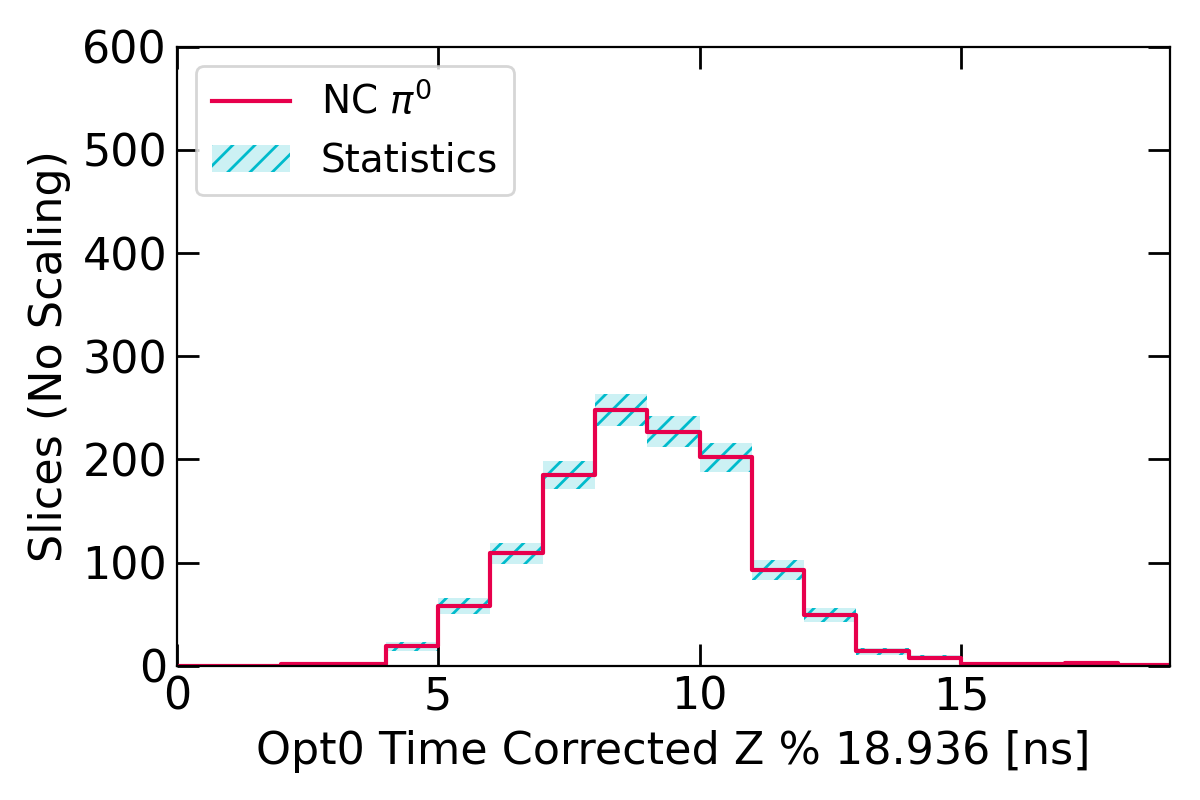
\includegraphics[width=\textwidth]{ncpi0_stats_error}
            \caption{Statistical}%
            \label{fig:bkg_stat}
        \end{subfigure}
        \hfill
        \begin{subfigure}[b]{0.495\textwidth}   
            \centering 
            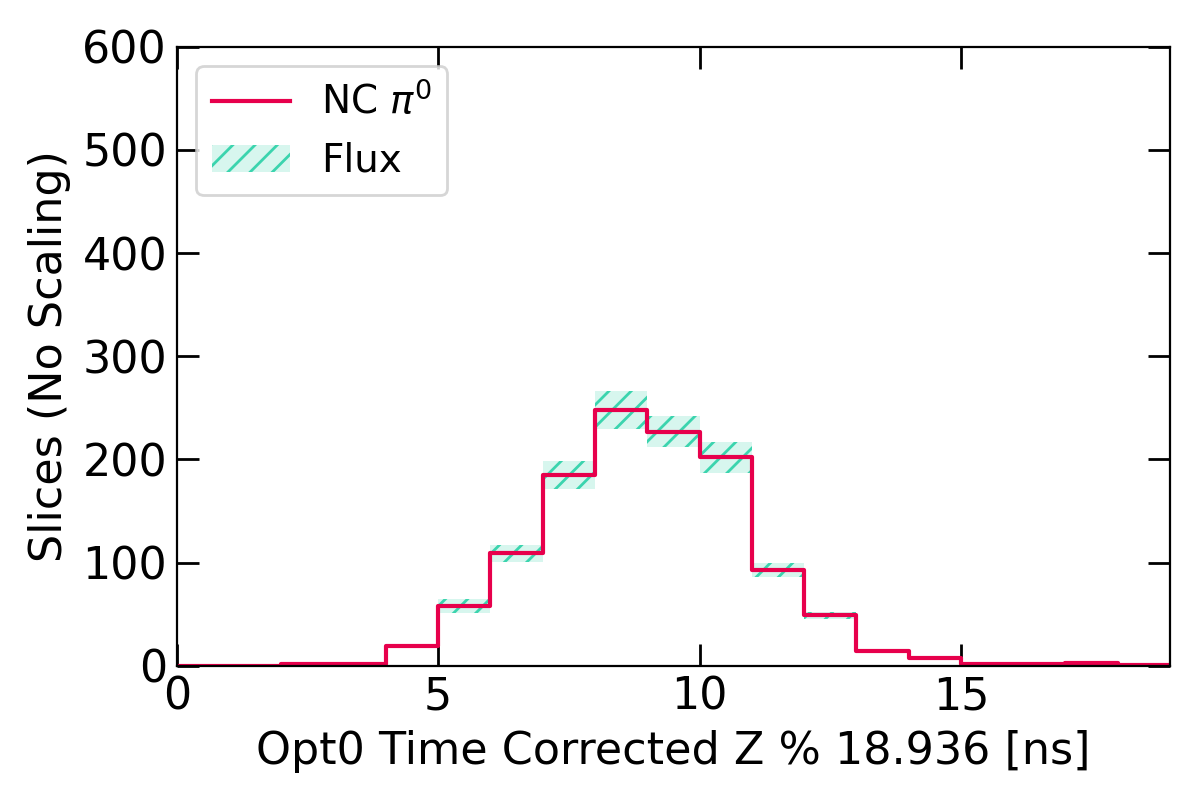
\includegraphics[width=\textwidth]{ncpi0_flx_err}
            \caption{Flux}%
            \label{fig:bkg_flux}
        \end{subfigure}
        \centering
        \begin{subfigure}[b]{0.495\textwidth}   
            \centering 
            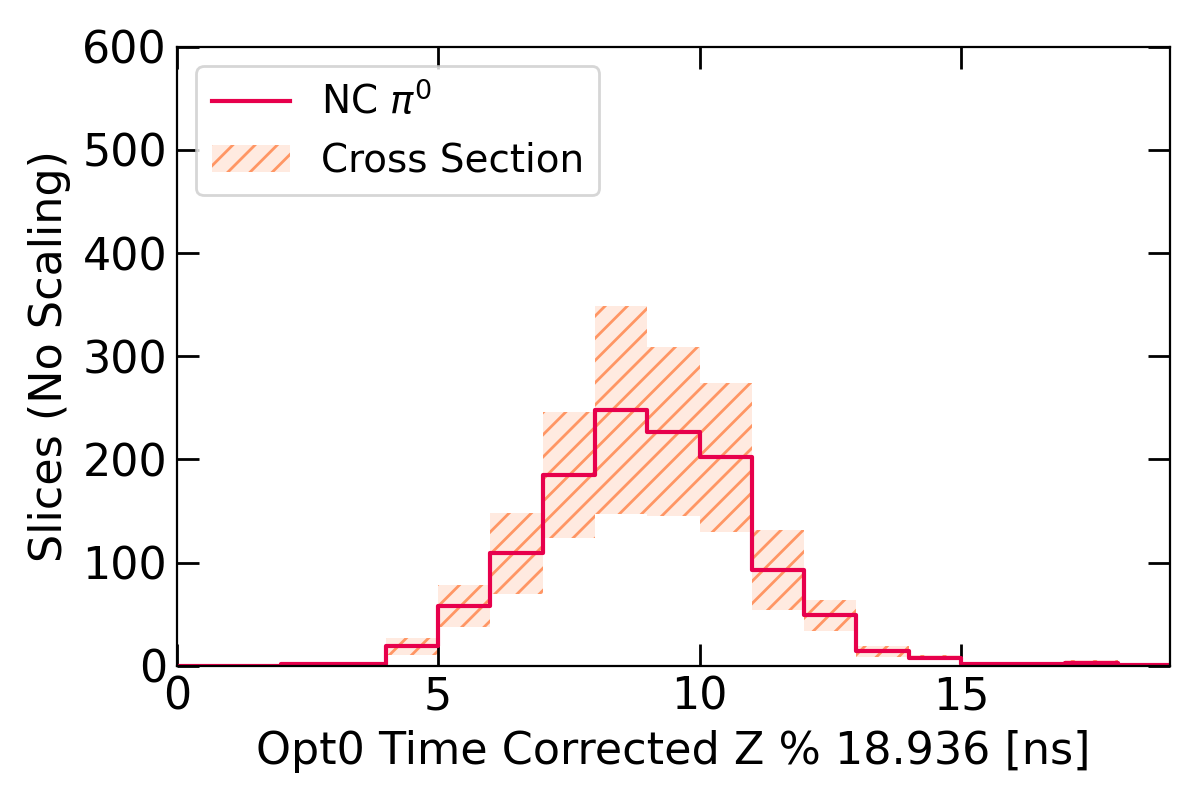
\includegraphics[width=\textwidth]{ncpi0_xsec_err}
            \caption{SM Neutrino Cross Section}%
            \label{fig:bkg_xsec}
        \end{subfigure}
        \caption{
	Plot showing different sources of uncertainty (bottom) of backgrounds.
	}
        \label{fig:bkg_error}
	\vspace{0.5cm}
%\end{figure}
%\begin{figure}[htbp!] 
\centering    
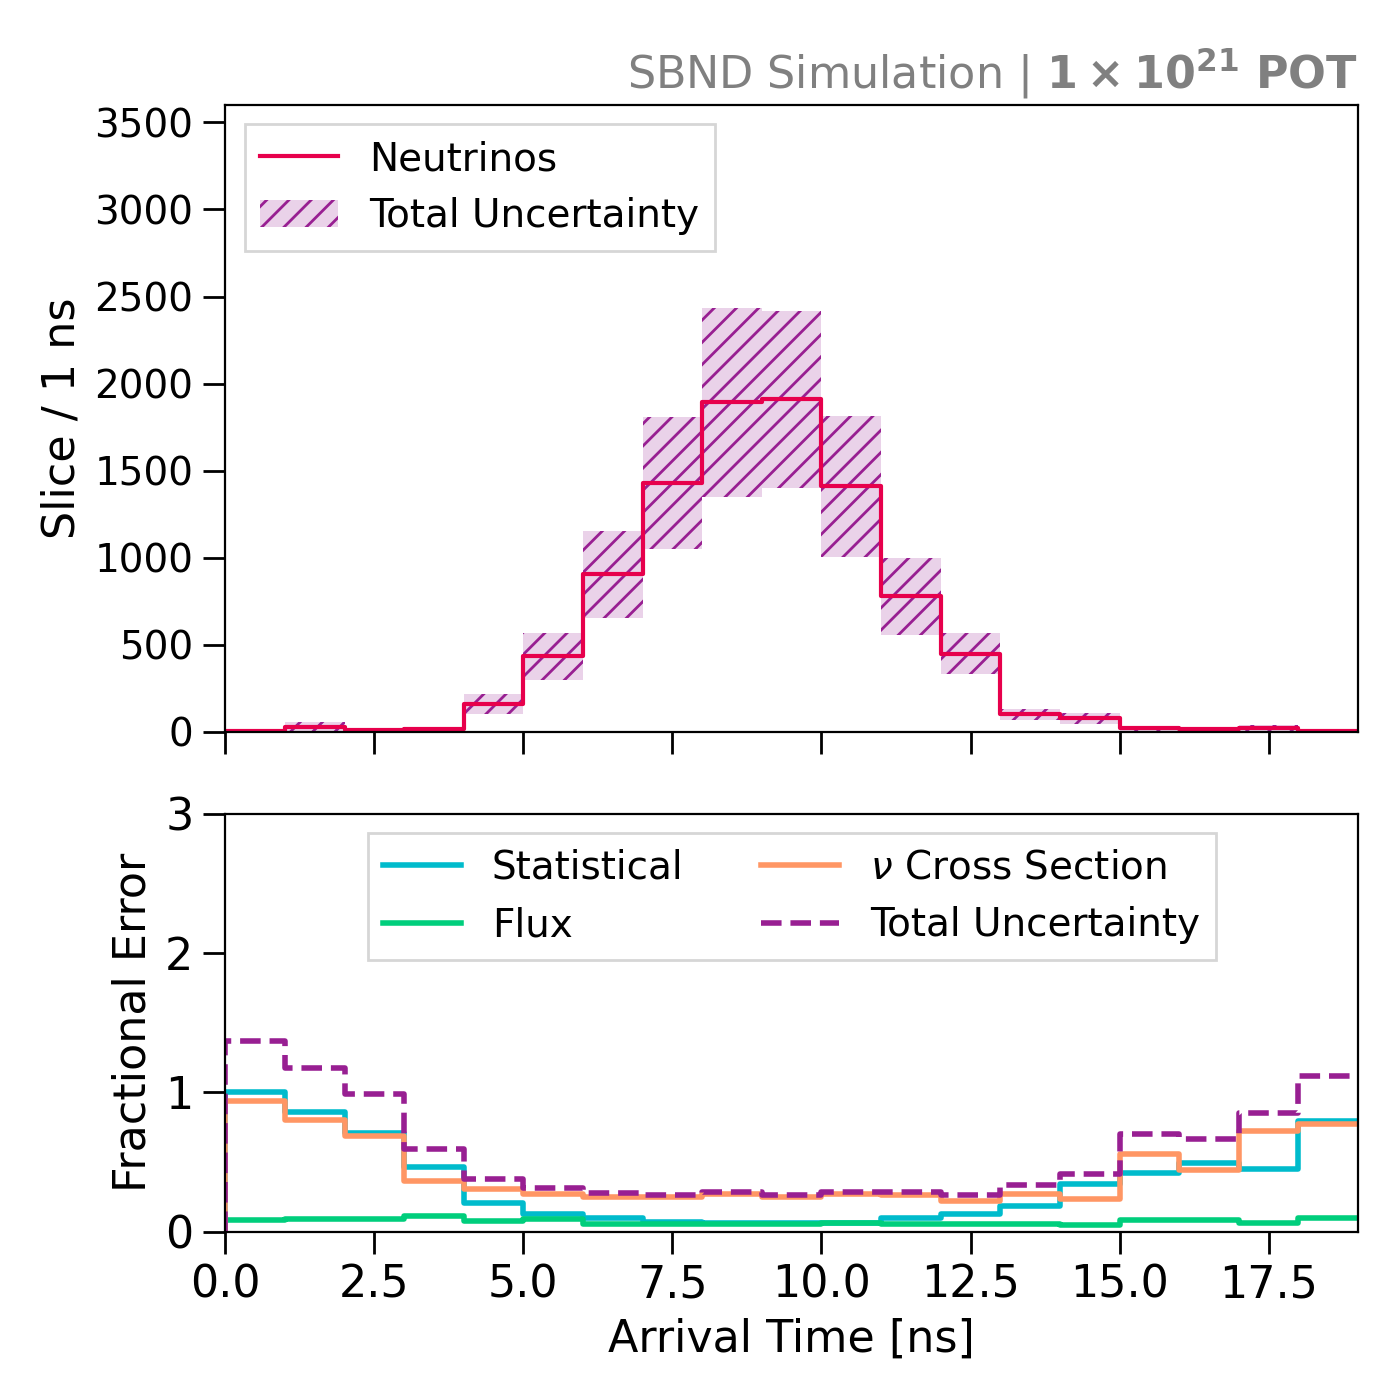
\includegraphics[width=0.5\textwidth]{bkg_error}
\caption[bkg_error]{
Plot showing the total uncertainty (top) and fractional uncertainties (bottom) of backgrounds.
}
\label{fig:bkg_total_error}
\end{figure}
%********************************** %First Section  **************************************

\section{Limits Setting Procedure}

\subsection{Hypothesis Definition}

\subsection{Likelihood-based Test Statistic}

\subsection{The CL$_{\mathrm{s}}$ Method}

\subsection{Computing Test Statistic Distributions}

\subsection{Setting The Upper Limits}
%********************************** %First Section  **************************************

\section{Results}

\subsection{Expected Limits on Majorana HNLS}

\subsection{Comparison With Other Experiments}

%********************************** %First Section  **************************************
\section{Concluding Remarks}
